\documentclass[11pt,a4paper]{article}
\usepackage[margin=0.6in]{geometry}
\usepackage{amsmath,amssymb}
\usepackage{tikz}
\usetikzlibrary{shapes.geometric,arrows.meta,positioning,calc,fit,backgrounds}
\usepackage{times}

\pagestyle{empty}

\begin{document}

\begin{center}
{\LARGE \textbf{3\quad Architecture Work Flow}}\\[1.2em]

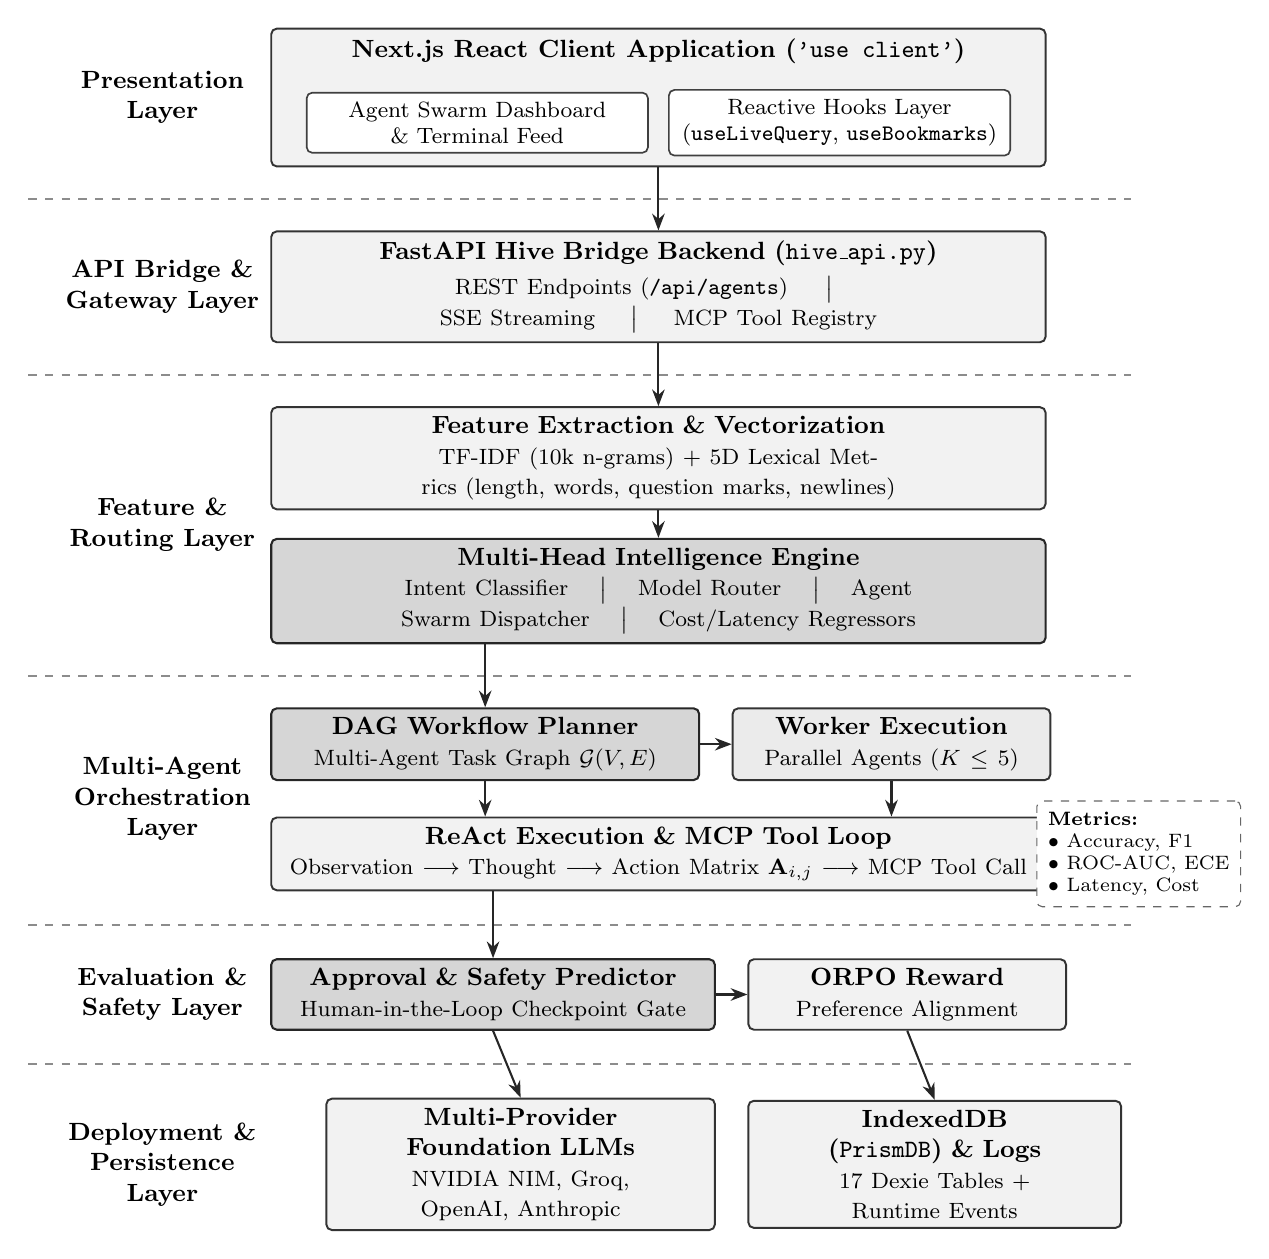
\begin{tikzpicture}[
    auto,
    font=\small,
    layer_label/.style = {
        font=\small\bfseries,
        align=center,
        text width=2.8cm
    },
    box/.style = {
        rectangle,
        draw=black!80,
        line width=0.7pt,
        fill=black!5,
        rounded corners=2pt,
        text width=9.2cm,
        minimum height=0.75cm,
        align=center,
        font=\small
    },
    subbox/.style = {
        rectangle,
        draw=black!75,
        line width=0.6pt,
        fill=white,
        rounded corners=2pt,
        text width=4.1cm,
        minimum height=0.7cm,
        align=center,
        font=\footnotesize
    },
    shaded/.style = {
        rectangle,
        draw=black!85,
        line width=0.75pt,
        fill=black!16,
        rounded corners=2pt,
        text width=9.2cm,
        minimum height=0.8cm,
        align=center,
        font=\small
    },
    arrow/.style = {
        -{Stealth[scale=0.95]},
        line width=0.75pt,
        draw=black!85
    },
    dashed_line/.style = {
        draw=black!45,
        dashed,
        line width=0.6pt
    }
]

    % Center X for main diagram column is at x=1.5
    % Left labels are placed at x=-4.8
    
    % =========================================================================
    % LAYER 1: PRESENTATION LAYER
    % =========================================================================
    \node [box, text width=9.6cm, minimum height=1.75cm] (box1) at (1.5, 0) {};
    \node [anchor=north, font=\small\bfseries, inner sep=4pt] at (box1.north) {Next.js React Client Application (\texttt{'use client'})};
    \node [subbox] (sub1a) at (-0.8, -0.32) {Agent Swarm Dashboard\\\& Terminal Feed};
    \node [subbox] (sub1b) at (3.8, -0.32) {Reactive Hooks Layer\\(\texttt{useLiveQuery}, \texttt{useBookmarks})};
    
    \node [layer_label] (lbl1) at (-4.8, 0) {Presentation\\Layer};

    % =========================================================================
    % LAYER 2: API BRIDGE & GATEWAY LAYER
    % =========================================================================
    \node [box, text width=9.6cm, below=0.8cm of box1] (box2) {
        \textbf{FastAPI Hive Bridge Backend (\texttt{hive\_api.py})}\\[0.2em]
        \footnotesize REST Endpoints (\texttt{/api/agents}) $\;\big|\;$ SSE Streaming $\;\big|\;$ MCP Tool Registry
    };
    \node [layer_label] (lbl2) at (-4.8, 0 |- box2) {API Bridge \&\\Gateway Layer};

    % Separator 1
    \coordinate (sep1) at ($(box1.south)!0.5!(box2.north)$);
    \draw [dashed_line] (-6.5, 0 |- sep1) -- (7.5, 0 |- sep1);

    % =========================================================================
    % LAYER 3: FEATURE & ROUTING LAYER
    % =========================================================================
    \node [box, text width=9.6cm, below=0.8cm of box2] (box3a) {
        \textbf{Feature Extraction \& Vectorization}\\
        \footnotesize TF-IDF (10k n-grams) + 5D Lexical Metrics (length, words, question marks, newlines)
    };
    \node [shaded, text width=9.6cm, below=0.35cm of box3a] (box3b) {
        \textbf{Multi-Head Intelligence Engine}\\
        \footnotesize Intent Classifier $\;\big|\;$ Model Router $\;\big|\;$ Agent Swarm Dispatcher $\;\big|\;$ Cost/Latency Regressors
    };
    \coordinate (c_layer3) at ($(box3a.center)!0.5!(box3b.center)$);
    \node [layer_label] (lbl3) at (-4.8, 0 |- c_layer3) {Feature \&\\Routing Layer};

    % Separator 2
    \coordinate (sep2) at ($(box2.south)!0.5!(box3a.north)$);
    \draw [dashed_line] (-6.5, 0 |- sep2) -- (7.5, 0 |- sep2);

    % =========================================================================
    % LAYER 4: MULTI-AGENT ORCHESTRATION LAYER
    % =========================================================================
    \node [shaded, text width=5.2cm, below=0.8cm of box3b, xshift=-2.2cm] (box4a) {
        \textbf{DAG Workflow Planner}\\
        \footnotesize Multi-Agent Task Graph $\mathcal{G}(V, E)$
    };
    \node [box, text width=3.8cm, fill=black!8, right=0.4cm of box4a] (box4b) {
        \textbf{Worker Execution}\\
        \footnotesize Parallel Agents ($K \le 5$)
    };
    
    \node [box, text width=9.6cm, below=0.45cm of box4a, xshift=2.2cm] (box4c) {
        \textbf{ReAct Execution \& MCP Tool Loop}\\
        \footnotesize Observation $\longrightarrow$ Thought $\longrightarrow$ Action Matrix $\mathbf{A}_{i,j}$ $\longrightarrow$ MCP Tool Call
    };
    
    \coordinate (c_layer4) at ($(box4a.center)!0.5!(box4c.center)$);
    \node [layer_label] (lbl4) at (-4.8, 0 |- c_layer4) {Multi-Agent\\Orchestration\\Layer};

    % Separator 3
    \coordinate (sep3) at ($(box3b.south)!0.5!(box4a.north)$);
    \draw [dashed_line] (-6.5, 0 |- sep3) -- (7.5, 0 |- sep3);

    % Metrics side-box positioned clearly on the right without overlapping
    \node [rectangle, draw=black!60, dashed, fill=white, rounded corners=2pt, font=\scriptsize, align=left, inner sep=4pt] (metrics) at (7.6, 0 |- box4c) {
        \textbf{Metrics:}\\
        $\bullet$ Accuracy, F1\\
        $\bullet$ ROC-AUC, ECE\\
        $\bullet$ Latency, Cost
    };

    % =========================================================================
    % LAYER 5: EVALUATION & SAFETY LAYER
    % =========================================================================
    \node [shaded, text width=5.4cm, below=0.85cm of box4c, xshift=-2.1cm] (box5a) {
        \textbf{Approval \& Safety Predictor}\\
        \footnotesize Human-in-the-Loop Checkpoint Gate
    };
    \node [box, text width=3.8cm, right=0.4cm of box5a] (box5b) {
        \textbf{ORPO Reward}\\
        \footnotesize Preference Alignment
    };
    
    \node [layer_label] (lbl5) at (-4.8, 0 |- box5a) {Evaluation \&\\Safety Layer};

    % Separator 4
    \coordinate (sep4) at ($(box4c.south)!0.5!(box5a.north)$);
    \draw [dashed_line] (-6.5, 0 |- sep4) -- (7.5, 0 |- sep4);

    % =========================================================================
    % LAYER 6: DEPLOYMENT & PERSISTENCE LAYER
    % =========================================================================
    \node [box, text width=4.7cm, below=0.85cm of box5a, xshift=0.35cm] (box6a) {
        \textbf{Multi-Provider Foundation LLMs}\\
        \footnotesize NVIDIA NIM, Groq, OpenAI, Anthropic
    };
    \node [box, text width=4.5cm, right=0.4cm of box6a] (box6b) {
        \textbf{IndexedDB (\texttt{PrismDB}) \& Logs}\\
        \footnotesize 17 Dexie Tables + Runtime Events
    };
    
    \coordinate (c_layer6) at ($(box6a.center)!0.5!(box6b.center)$);
    \node [layer_label] (lbl6) at (-4.8, 0 |- c_layer6) {Deployment \&\\Persistence\\Layer};

    % Separator 5
    \coordinate (sep5) at ($(box5a.south)!0.5!(box6a.north)$);
    \draw [dashed_line] (-6.5, 0 |- sep5) -- (7.5, 0 |- sep5);

    % =========================================================================
    % ARROWS WITH CLEAN INTER-NODE ATTACHMENT
    % =========================================================================
    \draw [arrow] (box1.south) -- (box2.north);
    \draw [arrow] (box2.south) -- (box3a.north);
    \draw [arrow] (box3a.south) -- (box3b.north);
    
    % From routing to planner & workers
    \draw [arrow] (box3b.south -| box4a.north) -- (box4a.north);
    \draw [arrow] (box4a.east) -- (box4b.west);
    
    % From planner & workers into ReAct loop
    \draw [arrow] (box4a.south) -- (box4a.south |- box4c.north);
    \draw [arrow] (box4b.south) -- (box4b.south |- box4c.north);
    
    % From ReAct loop into evaluation & safety
    \draw [arrow] (box4c.south -| box5a.north) -- (box5a.north);
    \draw [arrow] (box5a.east) -- (box5b.west);
    
    % From evaluation into foundation LLMs and persistence
    \draw [arrow] (box5a.south) -- (box6a.north);
    \draw [arrow] (box5b.south) -- (box6b.north);

\end{tikzpicture}

\vspace{1.5em}
{\Large \textbf{Figure 4.2: Different Layers.}}
\end{center}

\end{document}
